\documentclass{article}

\usepackage[T1]{fontenc}
\usepackage[utf8]{inputenc}
\usepackage{lmodern}
\usepackage{listings}
\usepackage[colorlinks = true,
            linkcolor = blue,
            urlcolor  = blue,
            citecolor = blue,
            anchorcolor = blue]{hyperref}
\usepackage{graphicx}
\usepackage{subfig}
\usepackage[dvipsnames,table,xcdraw]{xcolor}
\usepackage{array}
\newcolumntype{P}[1]{>{\centering\arraybackslash}p{#1}}
\newcolumntype{M}[1]{>{\centering\arraybackslash}m{#1}}
\author{Francesco Boi}
\title{Self-driving cars program - project  3: Traffic Signs Classifier}
\date{}

\let\cd\lstinline

\begin{document}
% Python style for highlighting

\maketitle
\tableofcontents 

\lstdefinestyle{customc}{
  belowcaptionskip=1\baselineskip,
  breaklines=true,
  %frame=L,
  xleftmargin=\parindent,
  language = Python,
  showstringspaces=false,
  basicstyle=\footnotesize\ttfamily,
  keywordstyle=\bfseries\color{blue!85!black},
  commentstyle=\itshape\color{gray},
  identifierstyle=\color{black},
  stringstyle=\color{red},
  numbers=left,                    				% where to put the line-numbers; possible values are (none, left, right)
  numbersep=5pt,                   			% how far the line-numbers are from the code
  numberstyle=\tiny\color{gray},     % the style that is used for the line-numbers
  stepnumber=1,
  tabsize=4,
}
\lstdefinestyle{customasm}{
  belowcaptionskip=1\baselineskip,
  frame=L,
  %xleftmargin=\parindent,
  language=[x86masm]Assembler,
  basicstyle=\footnotesize\ttfamily,
  commentstyle=\itshape\color{purple!40!black},
  stepnumber=1,
   tabsize=4,
}
\definecolor{lightgray}{rgb}{.9,.9,.9}
\definecolor{darkgray}{rgb}{.4,.4,.4}
\definecolor{purple}{rgb}{0.65, 0.12, 0.82}
\lstset{escapechar=ç,style=customc}


\section{Content of the project}
Here is the content of the project:
\begin{itemize}
\item \textit{writeup.pdf} (this file): report of the project;
\item \textit{writeup.tex}: tex source code for;
\item \textit{writeUpImgs}: folder containing the images shown in this document;
\item \textit{Traffic\_Sign\_Classifier.ipynb}: ipython notebook with the code for the classifier;
\item \textit{webSigns}: folder containing traffic sign images downloaded from the Web to test the NN on;
\item \textit{OtherStudentsImgs}: folder containing traffic sign images used by other students' projects to test the NN on.
\end{itemize}

Here is the link to the \href{https://github.com/FrancescoBoi/UdaciytySDC-TrafficSignsClassifier}{github project}.

\section{Project goals}
The steps of this project are the following:
\begin{itemize}
\item Download and load the dataset.
\item Explore, summarise and visualize the data.
\item Design, train and test a neural network.
\item Use the model to predict new images.
\item Analyse the softmax probabilities of the new images.
\item Show the activation of the hidden convolutional layers.
\end{itemize}

\section{Dataset summary and exploration}
The dataset consists of a training, validation and test set with the following characteristics:
\begin{itemize}
\item The size of the training set is $34799$.
\item The size of the validation set is $4410$.
\item The size of the test set is $12630$.
\item The shape of a traffic sign image is $(32,32,3)$.
\item The number of unique classes/labels in the data set is $43$.
\end{itemize}

The set sizes and images shape have been calculated using the \cd+shape+ attribute of the numpy arrays. The number of classes have been calculated in two ways: looking at the maximum value of \cd+y_train+ and adding $1$ and confirmed by using the \cd+numpy.unique+ function.
\begin{lstlisting}
n_classes = max(y_train)+1
unique, counts = np.unique(y_train, return_counts=True)
assert n_classes == len(counts)
\end{lstlisting}

\subsection{Visualisation}
\autoref{fig:dataset} shows some images of the dataset whereas \autoref{fig:histo} shoes the histograms of the classes on the training, validation and test set. Note two things: some images are of really bad quality; note also that the classes are not equally represented: class 0, 41 and 42 have really few smaples whereas class 1 and 2 are overrepresented, 10 times more than class 0 for example.
\begin{figure}
\centering
\subfloat[Speed limit of 20 Km/h sign]{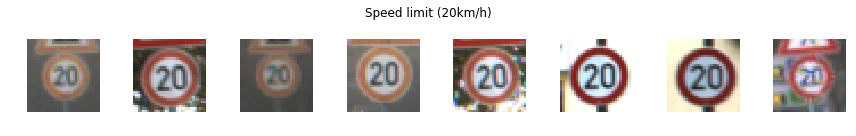
\includegraphics[width=0.8\textwidth]{writeUpImgs/20}\label{sign20}}\\
\subfloat[Stop sign]{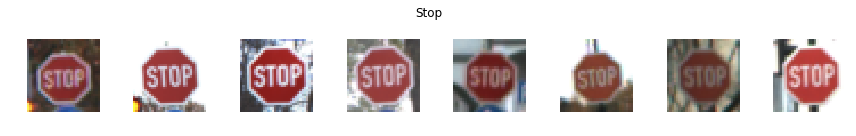
\includegraphics[width=0.8\textwidth]{writeUpImgs/stop}\label{stopSign}}
\caption{Example of images from the dataset.}
\label{fig:dataset}
\end{figure}

\begin{figure}
\centering
\subfloat[Histogram of the classes in the training set]{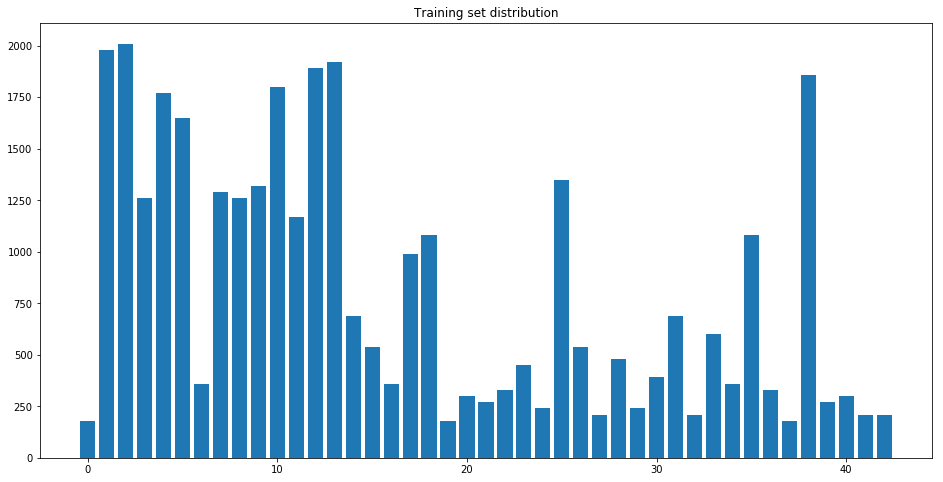
\includegraphics[scale=0.3]{writeUpImgs/histoTrain}\label{histoTrain}}\\
\subfloat[Histogram of the classes in the validation set]{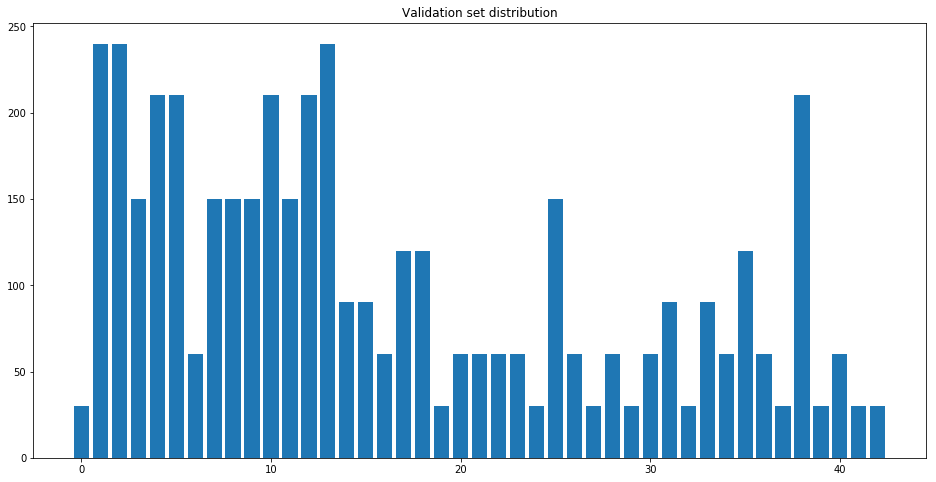
\includegraphics[scale=0.3]{writeUpImgs/histoVal}\label{histoValid}}\\
\subfloat[Histogram of the classes in the test set]{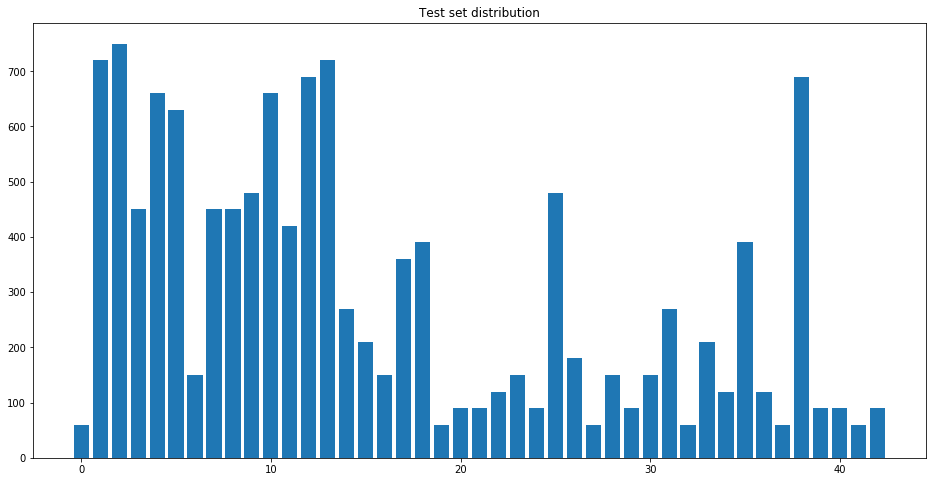
\includegraphics[scale=0.3]{writeUpImgs/histoTest}\label{histoTest}}
\caption{Example of images from the dataset.}
\label{fig:histo}
\end{figure}

\section{Design and test a model architecture}
\subsection{Preprocessing}
The preprocessing consists of two steps: converting the RGB images to grayscale and normalising the value between $-1$ and $1$ (almost $1$ actually, since $(255-128)/128$ is not $1$ exactly). Normalisation should improve and speed up the training process. Gray scale conversion should also speed up the training process since there are less parameters to train. Surprisingly, after running some trainings, it seems that the training process benefits from gray scale conversion. However, colours are very important in traffic sign recognition and a deeper network might take advantage of it.

Some gray scale images are shown in \autoref{fig:gray}

\begin{figure}
\centering
\subfloat[Speed limit of 20 Km/h sign in gray scale]{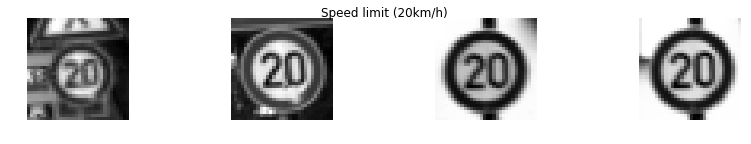
\includegraphics[width=0.8\textwidth]{writeUpImgs/20gray}\label{sign20gray}}\\
\subfloat[Stop sign in gray scale]{
\includegraphics[width=0.8\textwidth]{writeUpImgs/stopgray}\label{stopSigngray}}
\caption{Example of images from the dataset.}
\label{fig:gray}
\end{figure}

\subsection{Model}
The model architecture is the following:

\begin{tabular}{ |M{1.5cm}||M{1.5cm}||M{1.7cm}||M{1.7cm}||M{1cm}||M{1cm}|  }
 \hline
 \multicolumn{2}{|c|}{Neural network layers} \\
 \hline
Layer & Layer shape & Input shape & Output shape & Stride & Pad\\
 \hline
Input   & (32, 32, 1)&/&/&/&/\\
Conv &   (5,5,6) & (32,32,1) & (28,28,6)& (1,1)&valid\\
Relu &/&(28,28,6)&(28,28,6)&/&/\\
Max Pool & (2,2) & (28, 28, 6) & (14, 14, 6) & (2,2)&valid\\ 
Conv &   (5,5,16) & (14, 14, 6)& (10,10,16)& (1,1)&valid\\
Relu &/&(10,10,16)&(10,10,16)&/&/\\
Max Pool & (2,2) & (10,10,16) & (5, 5, 16) & (2,2)&valid\\
Flatten & / &(5,5,16) & (400) & /&/\\
Dropout &/ &(400) &(400) &/&/\\
Full & (120) & (400) & (120) & /&/\\
Relu &/&(120)&(120)&/&/\\
Dropout &/ &(120) &(120) &/&/\\
Full & (84) & (120) & (84) & /&/\\
Relu &/&(120)&(120)&/&/\\
Dropout &/ &(84) &(84) &/&/\\
Full & (10) & (84) & (10) &/&/\\
\hline
\end{tabular}

The softmax activation is called outside the \cd+LeNet()+ function as in the lecture.

To find a good set of hyper parameters, different models have been trained using a batch size of $128$ or $256$, a probabililty for the drop out layers of $0.5, 0.6, 0.7$ and 5 rates between $0.0001$ and $0.001$. Among these, the best result was with batch size $128$, rate $0.00055$ and probaility $0.7$. 

The number of epochs is $45$ but there is little to no improvement after $40$. Such a high number was chosen since a relatively small rate was used, hence the model kept improving. The Adam optimizer has been used. With this configuration I got a validation accuracy of $0.946$ and a test accuracy of $0.929$ (section \textit{Test accuracy} and \textit{Validation accuracy} in the notebook). On the training set the final accuracy is of $0.994$ so the model is slightly overfitting (section \textit{Training accuracy} in the notebook). 

Adding the dropout layer significantly improved training and validation accuracy since it prevents overfitting.

The LeNet architecture was used. This works quite well thanks to the convolutioal layers that are suitable for image applications. A convolutional layer uses less parameters than a fully connected layer and it allows to treat each region of the image equally since the parameters are the same.

\section{Test a model on new images}
\autoref{fig:webimgs} shows some images found on the Web.
\begin{figure}
\centering
\subfloat[Children crossing]{
\includegraphics[width=0.3\textwidth]{webSigns/resized/childrenRoadSignCropped}\label{web:childCross}}
\subfloat[Speed limit 20 Km/h]{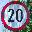
\includegraphics[width=0.3\textwidth]{webSigns/resized/RoadSign20}\label{web:20}}\\
\subfloat[Slippery road sign]{
\includegraphics[width=0.3\textwidth]{webSigns/resized/slipperyCropped}\label{web:slippery}}
\subfloat[Stop sign]{
\includegraphics[width=0.3\textwidth]{webSigns/resized/stop}\label{web:stop}}\\
\subfloat[Stop sign clean]{
\includegraphics[width=0.3\textwidth]{webSigns/resized/stop_clean}\label{web:stop_clean}}
\subfloat[Warning sign]{
\includegraphics[width=0.3\textwidth]{webSigns/resized/warningYellow}\label{web:warning}}\\
\subfloat[Wild animals sign]{
\includegraphics[width=0.3\textwidth]{webSigns/resized/wildAnimalsCropped}\label{web:wild_animals}}
\caption{Web images to test the neural network on.}
\label{fig:webimgs}
\end{figure}

\autoref{web:warning} might be difficult to classify because differently from the other training images, the sign has a yellow background instead of a white one, although the grayscale conversion might mitigate this. The other images look quite clean. \autoref{web:stop_clean} is not actually a picture but a digital representation of the sign. 


\subsection{Accuracy on web images}
The accuracy in this case is very poor, of $0.286$, infinitely worse than the test set. 

\autoref{fig:pred} shows the classification results. Only two classes are classified correctly: \autoref{web:stop_clean} as expected and \autoref{web:slippery}. The wild crossing sign is confused with the slippery road sign, which is unerstandable: they look very similar even to the human eye for such low resolution images. The general caution sign is not classified correctly, probably due to the yellow colour, but at least the NN recognised a triangular shape. The other stop sign (class 14) and the 20 km/h speed limit (class 0) are not classified correctly. Very likely, this is because these classes are underrepresented in the dataset. Especially for the 20 km/h sign, the class 30 km/h (class 1) is very similar but has roughly ten times more instances (see \autoref{fig:histo}), so the NN has learnt it has more chances of doing a better job by outputting class 1, since class 0 is very unlikely. In fact, this is exactly what it is doing: the 20 km/h speed limit is classified as th 30 km/speed limit.

Further analysis should include a confusion matrix and possibly compare the activation layers. Getting more instances of the underrepresented classes might be beneficial.

\section{Test a model on new images}
\autoref{fig:webimgs} shows some images found on the Web.
\begin{figure}
\centering
\subfloat{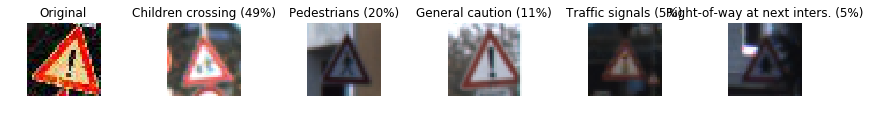
\includegraphics[width=0.9\textwidth]{writeUpImgs/webpred1}\label{web:pred1}}\\
\subfloat{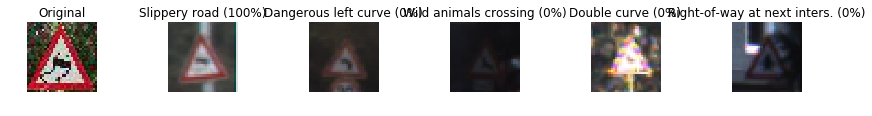
\includegraphics[width=0.9\textwidth]{writeUpImgs/webpred2}\label{web:pred2}}\\
\subfloat{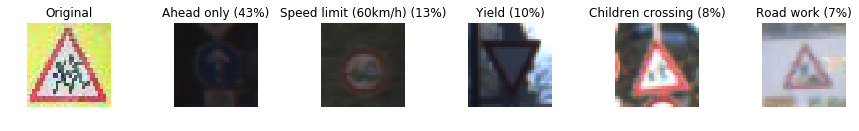
\includegraphics[width=0.9\textwidth]{writeUpImgs/webpred3}\label{web:pred3}}\\
\subfloat{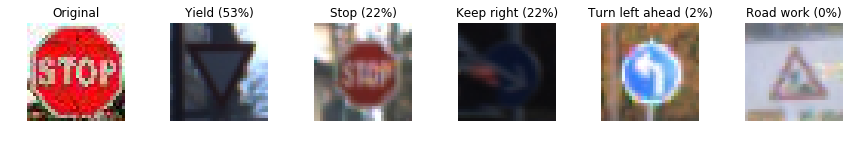
\includegraphics[width=0.9\textwidth]{writeUpImgs/webpred4}\label{web:pred4}}\\
\subfloat{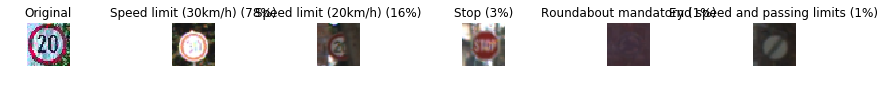
\includegraphics[width=0.9\textwidth]{writeUpImgs/webpred5}\label{web:pred5}}\\
\subfloat{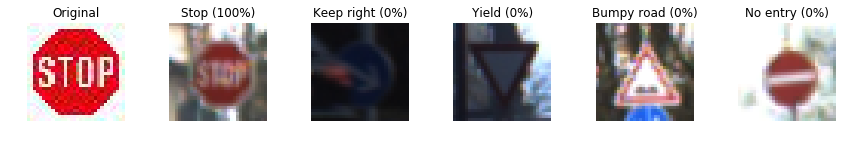
\includegraphics[width=0.9\textwidth]{writeUpImgs/webpred6}\label{web:pred6}}\\
\subfloat{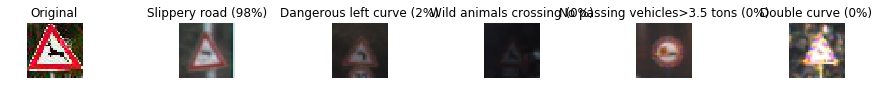
\includegraphics[width=0.9\textwidth]{writeUpImgs/webpred7}\label{web:pred7}}
\caption{Predictions on the new images.}
\label{fig:pred}
\end{figure}

\subsection{Accuracy on other students' images}
In the section \textit{Test on other students' images}, the NN has been tested on images used by other students for the same project. In this case the accuracy is $0.643$, which is signifiantly better than the previous one. Probably I have chosen some bad images to test the NN.

\section{Visualisation of the hidden layers}
\autoref{fig:conv} shows the activations of the convolutional layer. Note that some feature maps are not activated (at least for this input). The first layer seems to learn a general shape whereas the second layer seems to highlight some details in the image. The result of the first layer looks similar to different derivative filters: the image is still recognisable. The second layer seems to look for the diagonal arrow.
\begin{figure}
\centering
\subfloat[First conv layer]{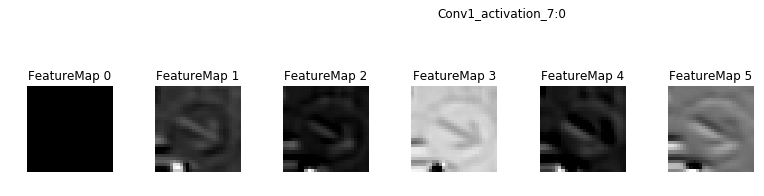
\includegraphics[width=0.9\textwidth]{writeUpImgs/conv1}\label{fig:conv1}}\\
\subfloat[Second conv layer]{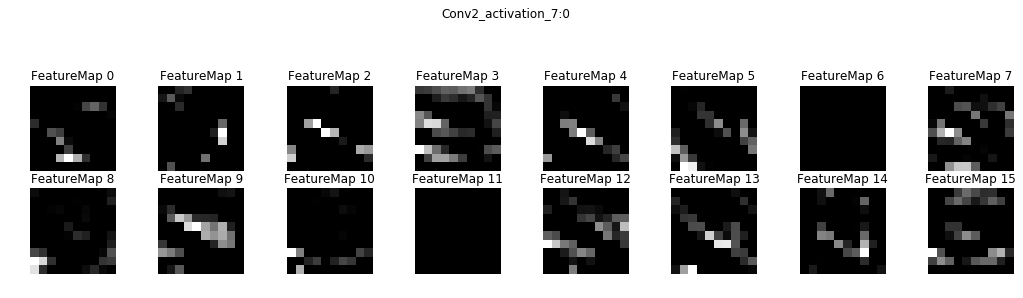
\includegraphics[width=0.9\textwidth]{writeUpImgs/conv2}\label{fig:conv2}}\\
\caption{Activations of the convolutional hidden layers.}
\label{fig:conv}
\end{figure}

\end{document}
